\chapter{Design of Cloud-SAP}

\chapterintro{ This chapter introduces the high-level design of Cloud-SAP, highlighting its core concepts and indicating possible implementation ideas.
}

\section{Requirements}
One can notice that elements that yields a solution for a problem stated in the first chapter, which is ensuring that users' application provide appropriate Quality-of-Service for its customers in a most-cost effective manner, were gradually introduced in previous chapters:

\begin{itemize}
	\item \emph{scalability} - ability to improve application performance by enriching resources
	\item \emph{adaptivity} - ability to adapt (i.e. scale) appropriately to a current usage pattern
	\item \emph{inter-cloud awareness} - ability to compose an application deployment using different cloud providers; cooperation with different cloud provider to supply application with extra resources while performing application scaling
\end{itemize}

Next section states the general overview of the proposed solution, while the consecutive sections details its elements and finally the last section summarises the design choices in a context of system requirements.
	
\section{High-level design}
\subsection{Overview}

\begin{figure}[!ht]
  \begin{center}
    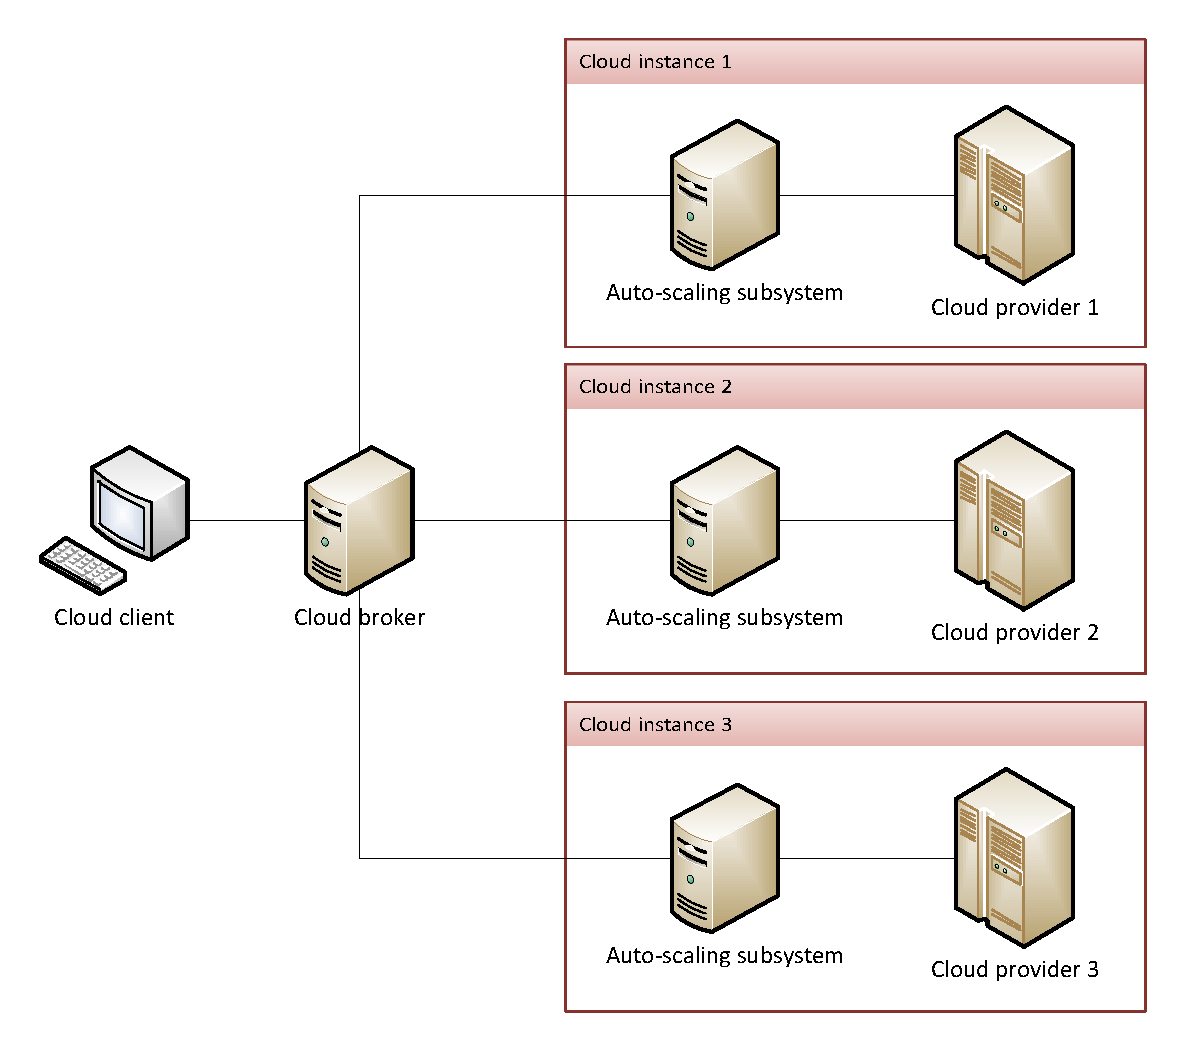
\includegraphics[width=0.8\textwidth]{chapter-5/hld-overview}
  \end{center}
  \caption{Cloud-SAP high level overview}
  \label{design:hld-overview}
\end{figure}

Diagram \ref{design:hld-overview} illustrates exemplary Cloud-SAP deployment, among depicted components we can distinguish two main parts of proposed solution: auto-scaling subsystem and inter-cloud broker. Auto-scaling subsystem is responsible for scaling users' application, taking into account different scalability perspectives, handled by a different layers:
\begin{itemize}
	\item application platform layer: application platform tuning
	\item container layer: vertical scaling
	\item stack layer: horizontal scaling
	\item inter-cloud layer: scaling out across different cloud providers
\end{itemize}
The last mentioned layer - inter-cloud - cooperates with different cloud providers, hence, it requires additional work to be done. In fact, these extra tasks are delegated to a inter-cloud broker, responsible for a dialog in a cloud federation.

\begin{figure}[!ht]
  \begin{center}
    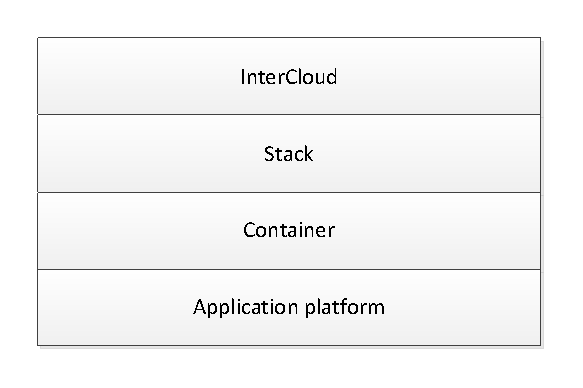
\includegraphics[width=0.5\textwidth]{chapter-5/sap-layers}
  \end{center}
  \caption{Layered structure of Cloud-SAP}
  \label{design:csap-layers}
\end{figure}

\subsection{Auto-scaling subsystem}

\subsubsection{Autonomic components}
Each layer of the Cloud-SAP (shown in figure \ref{design:csap-layers}) must be characterised by an ability to adapt to a given application usage. One of the first models that ensured system adaptivity is an autonomic component, concept based on a feed-back loop, initially proposed by IBM \cite{IBM06}. Figure \ref{design:autonomic-component} depicts that architecture. This observation is a foundation of proposed architecture - adaptivity is achieved by enriching each layer with an elasticity controller that is in fact an autonomic component.

\begin{figure}[!ht]
  \begin{center}
    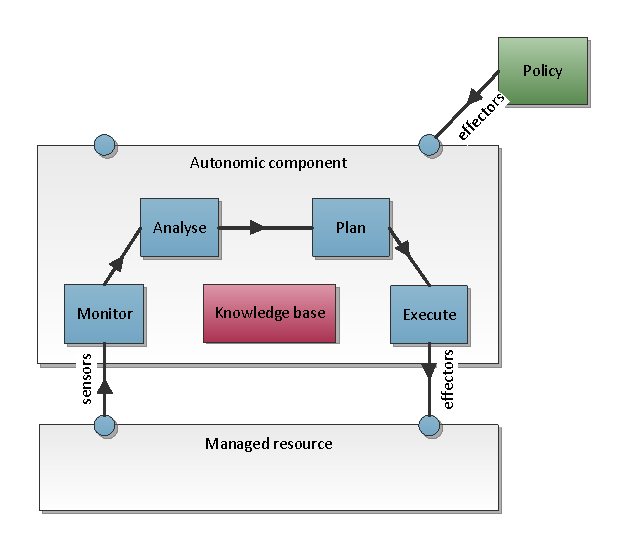
\includegraphics{chapter-5/autonomic-component}
  \end{center}
  \caption{autonomic component}
  \label{design:autonomic-component}
\end{figure}

Due to the fact that designed platform operates on multiple layers, we can extend idea of an autonomic component by using concept of a multi-hierarchical autonomic system \cite{LiWoZh05}. Figure \ref{design:hierarchical-autonomic-system} illustrates that hierarchy, were each level represents a different perspective on an application scaling. First three hierarchy levels (application tuning, container, stack) are centralised and controlled by a single elasticity controller at each level, while the last inter-cloud level is a decentralized one - each cloud instance is fully independent.

\begin{figure}[!ht]
  \begin{center}
    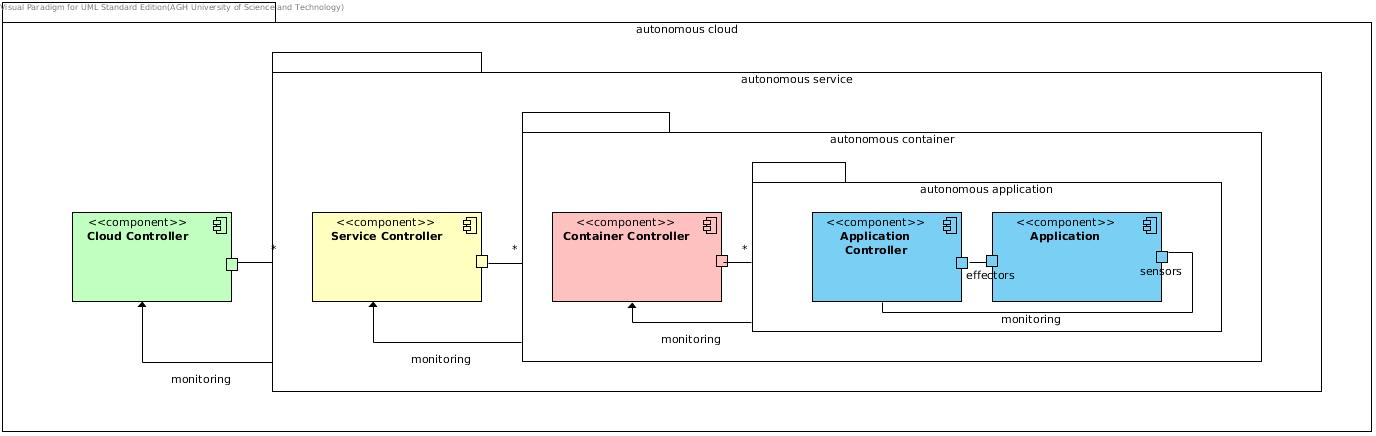
\includegraphics[width=0.8\textwidth]{chapter-5/hierarchical-autonomic-system}
  \end{center}
  \caption{Cloud-SAP as an hierarchical autonomic system}
  \label{design:hierarchical-autonomic-system}
\end{figure}

Considering hierarchy of our architecture, each level manages an underlying autonomic component, while being managed by an upper layer at the very same time.

\subsubsection{Monitoring}
Monitoring module of each elasticity controller aims to gather data from \textit{Sensors} of a managed resource. While design of Cloud-SAP doesn't have any specific requirements regarding underlying monitoring mechanism, there are a few aspects that should be taken into consideration. Table \ref{tab:monitoring-module-issues-summary} summarises main points.

\begin{table}[!htbp]
\begin{tabularx}{\textwidth}[]{ X X X }
\specialrule{.1em}{.05em}{.05em}
 & \textbf{Advantages} & \textbf{Disadvantages} \\ \specialrule{.1em}{.05em}{.05em} 

 
\textbf{data exchange model} & & \\ \specialrule{.1em}{.05em}{.05em}
push based &
-- notification driven: all changes are reflected immediately in the system
&
-- requires additional agent at monitored component
\\ \hline
pull based & 
-- more calculations are being done at monitoring module side (doesn't involve additional load at managed component)
& 
-- some monitoring cycles can be redundant if scheduler is not properly tuned
\\ \hline

\textbf{data format} & & \\ \specialrule{.1em}{.05em}{.05em}
binary &
-- space-effective
& 
-- unreadable for human
\\ \hline
character-based &
-- human readable
&
-- ineffective in terms of space
\\ \hline

\textbf{communication protocol} & & \\ \specialrule{.1em}{.05em}{.05em}
vendor specific &
-- provides specific data to a given managed component (ie. virtual machine / container)
& 
-- may cause incompatibility problem while expanding cloud-sap system to a consecutive cloud instances
\\ \hline
standard-based &
-- supports scaling across multiple cloud instances as long as they support standard
&
-- gathered data may be inadequate to a specific needs
\\ \hline
\end{tabularx}

\caption{Monitoring - summary of issues}
\label{tab:monitoring-module-issues-summary}

\end{table}

Cloud-SAP is entirely focused on further data processing, consequently decision whether to store monitoring data or not is entirely implementation dependent.

\subsubsection{Analysis}
Analyse module applies a specified mathematical model to a gathered data and yields a conclusion on top of that. There is a vast number of models that can be used for that purpose, for example \cite{LiWoZh05} enumerates:
\begin{itemize}
 \item Queue-based Performance Models
 \item Dynamic models
 \item Monotonic static models
 \item Policy based models
\end{itemize}

It is vital that Cloud-SAP implementation use predictive approach \cite{JiPeLiCh11} and track changes \cite{ZhYaWo05} in a system, giving a solid foundation for a knowledge base that can contribute to a better data analysis in future.

\subsubsection{Planning}
Planning module is responsible for scheduling actions that have to be taken to solve problems reported by an earlier analysis. This may involve:
\begin{itemize}
 \item reserving some resources (for example to deploy a new virtual machine)
 \item handling situation where multiple entities compete about the resources (for example taking service's priority into account)
\end{itemize}

It is possible, however, that resolving issues is not possible at a current layer. It that case, the upper-layer is responsible for handling it.

\subsubsection{Execution}
It is expected that execution module manage resource by performing various operations on resource's effector. Each layer is characterised by different actions that can be taken, for example: application server reconfiguration, vertical or horizontal scaling. 

Enforcing actions on a managed component can be done using different methods, however, all of them requires an agent installed in a managed resource. Cloud-SAP does not enforce any specific technology, leaving low-level decision to an implementation.

\subsubsection{Knowledge base}
Knowledge base is represented as a set of rules, policies shared across autonomic components.

-- TODO przyklad z ibma

\subsection{Cloud federation}
Opis najwyzej warstwy, ze ma brokery, wykorzystuje kilka chmur.


\section{Auto-scaling module}

\subsection{Application platform layer}

\subsection{Container layer}
Among the currently available monitoring systems remarkable are Cloud Watch \cite{CloudWatch}, OpenNebula (Information Manager / Virtual Machine Manager) \cite{OpenNebula} there are also open approaches such as Ganglia Monitoring System \cite{MaChCu04}.

\subsection{Stack layer}

\subsection{Cloud layer}


\section{Cloud federation}

\section{Solution discussion}
